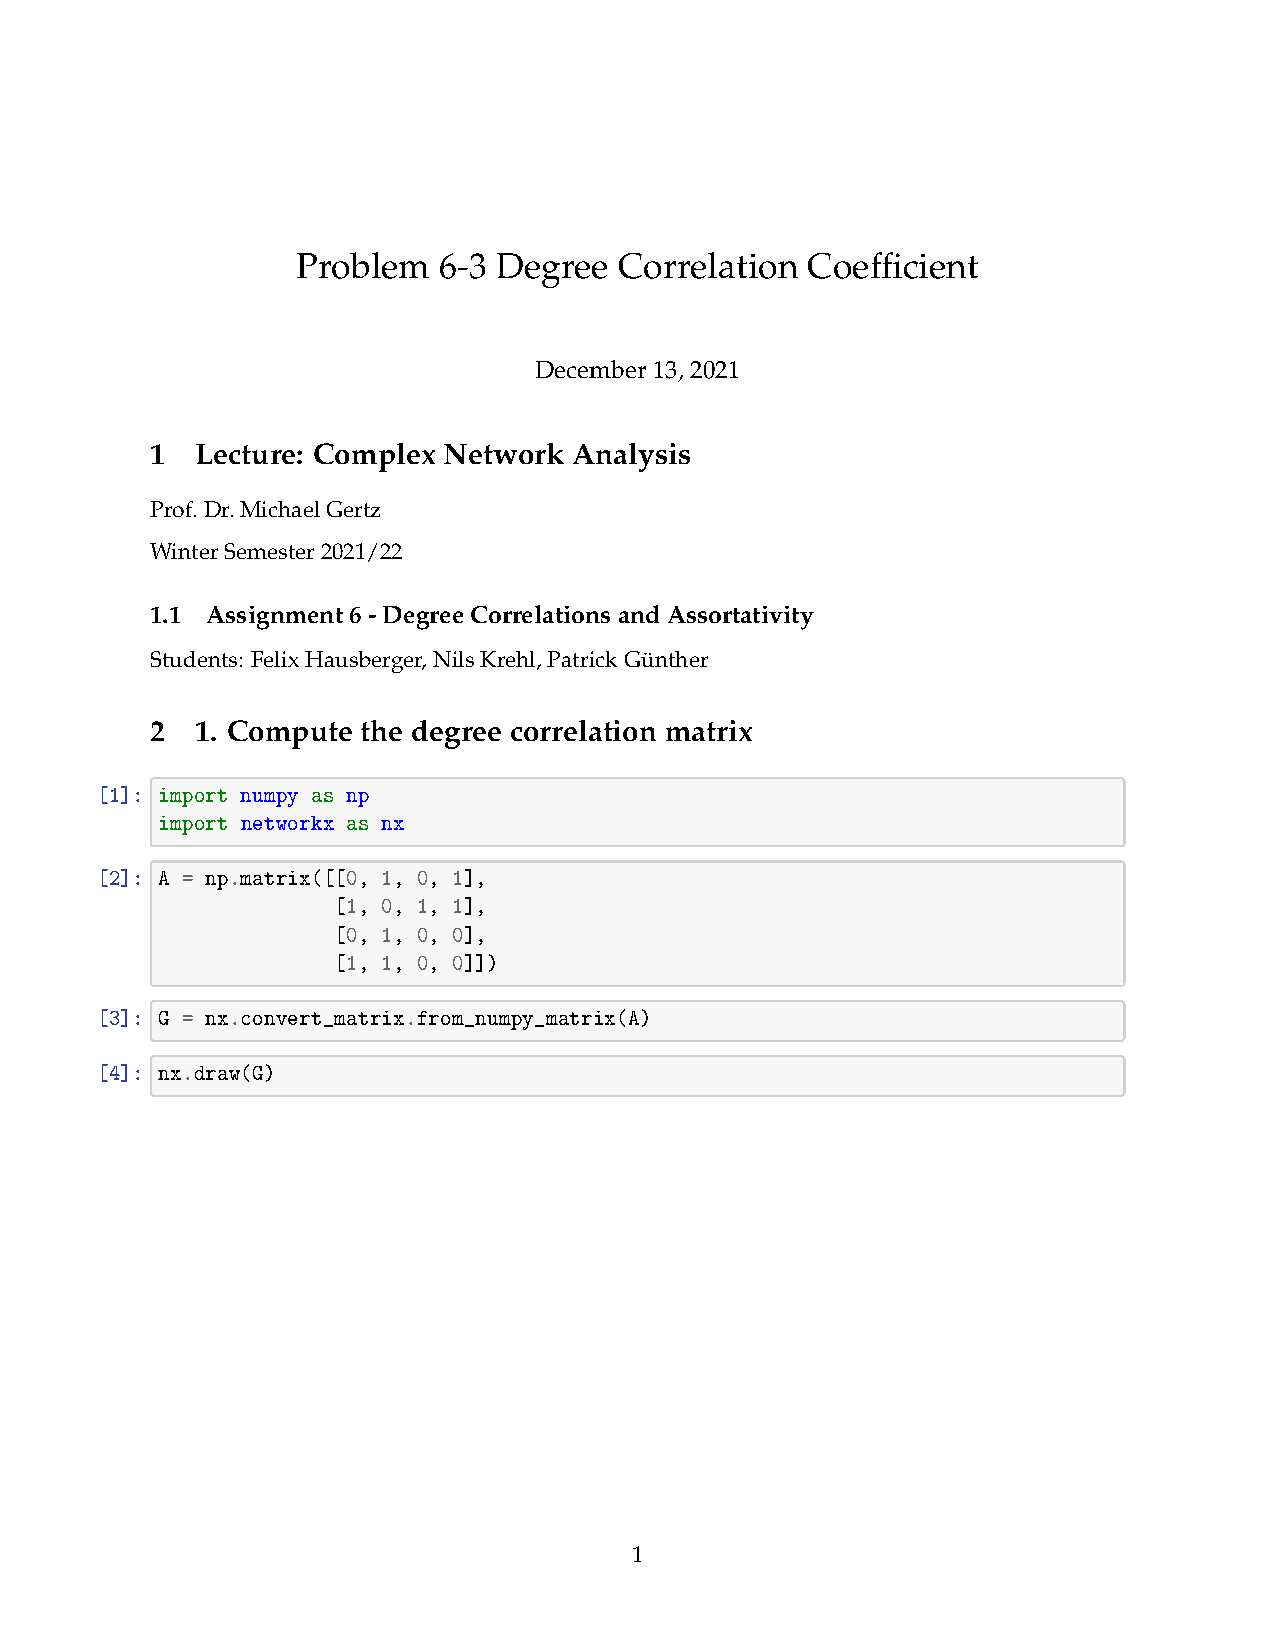
\includepdf[pages=-]{pdfs/problem_3.pdf}

\begin{enumerate}
	\item Compute the modularity of the graph.
	\begin{itemize}
		\item $L = 15$
		\item $n = 10$
		\item $n_c = 3$
		\item $L_A = 5 ; L_B = 2 ; L_C = 3$
		\item $k_A = 3 + 3 + 3 + 4 = 13 ; k_B = 2 + 4 + 3 = 9 ; k_C = 3 + 2 + 3 = 8$
	\end{itemize}
	
	Plugging this values into the given equation, we get $M(G,C) = 0.318$.
	
	\item Give proof that for every partitioning of every simple graph, it always holds that $M \leq 1$.
	
	For each component, its links within itself can be at most $L_c = L$. In this case, the component would hold all the links of the graph. For this component $\frac{L_c}{L}$ would be 1.  Since there is the term $\frac{k_c}{2L}^2$ subtracted from that, the summand for this component in the equation cannot be greater than 1. All other components remaining in the graph cannot have any links, which means that these are just unconnnected single nodes.  This means that their summand in the equation (ignorring the division by zero) would be 0. The whole equation thus cannot be greater than 1.
	
	For other cases where there are multiple components containing links, the total number of $L_c$ for all components is still limited by $L$. Thus it has to hold that $\sum^{n_c}_{c=1}(\frac{L_c}{L}) \leq 1$. Since the other term in each summand ($\frac{k_c}{2L}^2$) can only decrease the overall sum, $M \leq 1$ has to hold.
	
	For the trivial case of all nodes being disconnected, $M = 0$ (ignoring the division by 0).
	
\end{enumerate}